\chapter{Foundations of Light Transport Simulation}
\label{sec:foundations}

This chapter gives an overview on light transport simulation in the context of rendering in computer graphics and highlights the category of deterministic spherical harmonics based methods. Subsequent to the introduction and explanation of the physical background and important terminology, a brief overview over the landscape of methods for solving light transport problems is given. This is divided into three sections as per the following categorization: analytical methods (section~\ref{sec:foundations_analytical}), non-deterministic methods (section~\ref{sec:foundations_mc}) and deterministic methods (section~\ref{sec:foundations_deterministic}).

The field of computer graphics is primarily concerned with the generation of images from virtual scenes as seen by a virtual camera. This requires to reproduce the emission of light and its interaction with the scene and the sensor. The study of the behaviour of light is subject to optics, a seperate branch of physics. Due to the intricate nature of light, a series of increasingly complex models exist, which can account for various properties. Fundamental to light is its particle-wave duality, which states that light can be described both, as individual particles (photons) or waves. Challenging to the subject is, that not all properties of light can be described by solely the particle nor the wave perspective. To account for all properties, both have to be considered and require quantum mechanics. The field of wave optics is a simpler model that can account for optical effects, caused by the wave property, such as interference and diffraction. The simplest is provided by geometric optics, which models light as particle trajectories or rays and is referred to as ray optics. This model works well, when the wavelength is small compared to the scene the light propagates. 

As the virtual (and real) camera is supposed to capture the image as closely as possible to human perception, the simulated wavelength of light is limited to the visible range of a human being (390 to 700 nanometers). Because this is very small compared to distances encountered in real world scenes, wave effects are of less importance and geometric optics are sufficient most of the time. It is the basis for light transport simulation in graphics. This thesis is exclusively concerned with light transport in participating media i.a. clouds, smoke, fire and water.


% ============================================================
\section{The Radiative Transfer Equation}

With geometric optics light is described as particles, which travel through the scene along straight lines between single interactions. At each interaction the particle may change its course and continue to travel along another straight segment. When interacting with a medium, such as a cloud, each particle undergoes numerous interactions and creates complex overall trajectories based on medium properties.

To derive a model which can explain this complex system of many particles interacting with the scene, a statistical approach is taken. Since photons carry energy, a collection of photons can be described by their collective energy. To express the propagation of photons, time is required. This is captured by the quantity flux $\psi$: it gives the amount of energy from all photons going through a surface within a time interval and changes position and direction in space. It is given in Watts, which is specified in Joule (Energy) per second:
\begin{align*}
\psi\left(\vec{x}, \omega\right)
\quad
\left[\si{\watt} = \frac{\si{\joule}}{\si{\second}}\right]
\end{align*}

To find the flux for arbitrary surfaces (e.g. the camera sensor) and directions (e.g. the viewing direction of an observer), the radiance field $L$ is required. It captures the amount of light going through an infinitesmial small area and arriving from an infinitesimal small opening angle around a given direction $\omega$. More precisely, it specifies the change of flux according to a change in direction $\omega$ and a change in surface area that is projected onto a plane perpendicular to direction $\omega$:
\begin{align*}
L\left(\vec{x}, \omega\right) = \frac{\partial\partial\psi\left(\vec{x}, \omega\right)}{\partial\omega\partial A^\perp\left(\vec{x}\right)}
\quad
\left[\frac{\si{\watt}}{\si{\steradian} \si{\meter}^2}\right]
\end{align*}
The radiance field allows to find the amount of energy going through arbitrary surfaces and arbitrary angles by integration. This yields additional derivative quantities such as the fluence $\phi$, which integrates the radiance field over solid angle of the unit sphere at position $\vec{x}$:
\begin{align*}
\phi\left(\vec{x}\right) = \int_\Omega L\left(\vec{x}, \omega\right) \ud\omega
\quad
\left[\frac{\si{\watt}}{\si{\meter}^2}\right]
\end{align*}
It gives the total power of radiant energy arriving at position $\vec{x}$ from all directions. Integrating the radiance field after projecting it onto the planes of the cartesian coordinate system, gives rise to the flux vector $\vec{E}$:
\begin{align*}
\vec{E}\left(\vec{x}\right) = \int_\Omega L\left(\vec{x}, \omega\right)\omega \ud\omega
\end{align*}
The direction of the vector specifies the direction of bulk or dominant energy flow and the magnitude the net flux through an infinitesimal small surface, which is aligned to the direction.

The radiance field $L$ describes the distribution of photon densities in the scene and can easily be used to generate images by integrating it over the sensor surface of a virtual camera sensor and over all directions, from which photons can arrive on the sensor. This results in the energy that the sensor receives over a certain time (flux $\psi$).

%\TD{pixel color as integral over sensor surface}

However, the model needs to describe changes in the radiance field $L$ through changes in position. For this purpose, using the directional derivative $\left(\omega\cdot\nabla\right)L$ is used. It describes the rate of change of the radiance field $L$, when changing the position an infinitesimal step into direction $\omega$.

The radiance field $L$ changes along direction $\omega$ due to different optical phenomena, such as absorption, scattering and emission. Absorption models the effect of radiative energy being transformed into heat or kinetic energy. The amount of absorption depends on the medium and is controlled by the absorption coefficient $\sigma_a$. This value combines the number of absorbing particles in the medium as well as the collective surface area of their intersection with a hypothetical plane, which is oriented into the direction of change. The particles are assumed to be spherical or to have a random distribution of orientation. The coefficient controls the loss of energy due to absorption, when making an infintesmial step into direction $\omega$:
\begin{align}
\left(\omega\cdot\nabla_{a}\right)L = -\sigma_a L\left(\vec{x}, \omega \right)
\end{align}

\begin{figure}[t]
\centering
%\missingfigure{visualization of inscattering, outscattering and absorption.}
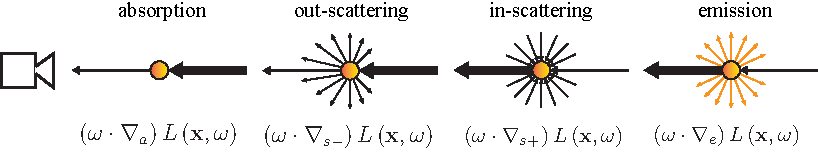
\includegraphics[width=1.0\textwidth]{03_foundations_of_light_transport_simulation/figures/fig_rte_terms.pdf}
\caption{Directional derivatives of the radiance $L$ along direction $\omega$ model the interaction of light with participating media and constitue the radiative transfer equation.}
\label{fig:rte_change_L_all}
\end{figure}


Scattering is an effect when photons collide with medium particles. They are not absorbed, but changed in their direction. This is controlled similarly to absorption by the scattering coefficient $\sigma_s$. Scattering has an effect on $L$ in two ways. Firstly, most of the scattering photons will change their direction away from the direction along which the rate of change of $L$, namely outscattering is measured:
\begin{align}
\left(\omega\cdot\nabla_{s-}\right)L = -\sigma_s L\left(\vec{x}, \omega \right)
\end{align}

Secondly, scattering affects the way the radiance field changes along $\omega$ in that photons arriving from all directions will collide with the volume and scatter into the direction $\omega$. This is called inscattering:
\begin{align}
\left(\omega\cdot\nabla_{s+}\right)L = \sigma_s \int_{\Omega'}p\left(\vec{x}, \omega'\cdot\omega\right)L\left(\vec{x}, \omega \right)\ud\omega'
\label{eq:rte_inscattering}
\end{align}
The quantity $p$ is the phase function, a medium parameter, which determines how light is redistributed from an incident direction $\omega'$ to the outgoing direction $\omega$. Since medium particles are assumed to either be spherical or randomly oriented, this function does not change as both vectors $\omega_i$ and $\omega$ are rotated, and therefore the cosine of the angle between the two vectors fulfills as a parameter.

%\todo[inline]{phase function}
%\todo[inline]{isotropic phase function}
%\todo[inline]{anisotropic phase function}
%\todo[inline]{mean cosine}
%\begin{align}
%\label{eq:foundations_mean_cosine}
%X
%\end{align}

Finally, the radiance field changes along direction $\omega$, due to the medium emitting photons itsself into direction $\omega$. This is modelled by a source term $Q_e$:
\begin{align}
\left(\omega\cdot\nabla_{e}\right)L = Q_e\left(\vec{x}, \omega\right)
\end{align}

All terms combined produce the radiative transfer equation (RTE), which expresses the change of the radiance field $L$, with respect to an infinitesimal change of position in direction $\omega$ at point $\vec{x}$ due to absorption, scattering and emission:
\begin{align}
\left(\nabla\cdot\omega\right)L\left(\vec{x}, \omega \right)
=&
-\sigma_t\left(\vec{x}\right) L\left(\vec{x}, \omega \right)\nonumber\\
&
+\sigma_s\left(\vec{x}\right) \int_{\Omega}
{
p\left(\omega'\cdot\omega\right)L\left(\vec{x}, \omega' \right)\ud\omega'
}
\label{eq:rte}
\\
&
+Q_e\left(\vec{x}, \omega\right)
\nonumber
\  .
\end{align}
with $\sigma_t=\sigma_a+\sigma_s$ being the extinction coefficient, which combines absorption and outscattering.

The radiative transfer equation, as presented, is based on important key assumptions about the modelled light transport (D'Eon~\cite{DEon14}):
\begin{itemize}
\item Linear transport: levels of heat, created by the absorption events don't measurably change the properties of the medium itself. Further photons do not collide with each other and therefore, the transport equations remain linear.
\item Steady-state: It is not of relevance to know how light propagates through the scene over time. The typical exposure times of cameras or the human visual system is in a regime, where it is safe to assume that sinks and sources are constant in time and are balanced out in an equilibrium state, such that the radiance field $L$ does not change over time.
\item Monoenergetic: often referred to as gray problems. Light is assumed to have a single frequency and color is introduced by solving the single frequency problem multiple times for color space primaries.
\item Energy-conserving media: the medium will never scatter more energy at any point, than it receives.
\item Scalar radiative transfer: polarization of light is not considered.
\item Uncorrelated interaction events: particles have no memory and the probability distribution of an interaction event does not depend on the previous interaction in any way (Moon et al.~\cite{Moon07}).
\item Isotropic medium: the medium is assumed isotropic, which means that absorption and scattering coefficients are not direction dependent and the phase function only depends on the cosine of the angle between incident and outgoing direction (Jakob et al.~\cite{Jakob10}).
\end{itemize}

For notational convenience and for developing the theory for deterministic methods, the radiative transfer equation is expressed in operator notation where transport, collision, and scattering are operators $\mathcal{T}$, $\mathcal{C}$ and $\mathcal{S}$, being applied to the radiance field $L$:
\begin{align}
\mathcal{T}\left(L\right) = -\mathcal{C}\left(L\right) + \mathcal{S}\left(L\right) + Q_e
\label{eq:rte_operator_notation}
\end{align}

Light transport simulation is the process for finding the solutions to $L$. Either for specific values of $\vec{x}$ and $\omega$ or globally. The following section gives an overview over the three main categories of methods for solving the radiative transfer equation, of which the last covers deterministic methods and leads into the subject of this thesis. The next section briefly covers analytical solutions which are popular and have been used to great effect. Section~\ref{sec:foundations_mc} covers non-deterministic methods, such as the Monte Carlo method. These methods will be introduced to motivate the need for deterministic methods as a potential means that boosts convergence of non-deterministic techniques. The last section introduces deterministic methods and covers how discretization of spatial and angular variable leads to a linear systems of equations.

% ============================================================
\section{Analytical Solutions}
\label{sec:foundations_analytical}

Analytical solutions to the radiative transfer equation exist for some very basic canonical problems, of which the point source problem is the most popular. It assumes an homogeneous medium (spatially constant $\sigma_t$) with infinite extent. For this problem, a correct analytical solution exists (D'Eon et al.~\cite{dEon11}). D'Eon also introduced a very accurate approximation by Grosjean~\cite{Grosjean56}, which is simpler to evaluate and convergent. This analytical solution will be used to verify the various methods developed as part of this thesis.

Pegoraro et al.~\cite{Pegoraro11} introduced a method based on the analytical solution to the point source problem for application in realtime rendering of single scattered light in participating media (termed airlight integral).

Jensen et al.~\cite{Jensen01} introduced the diffusion theory and in particular the analytical solution to the diffusion approximation for the point source problem (theoretical treatment in chapter~\ref{sec:diffusion_approximation}). In addition the authors introduced the method of images, which yielded an analytical solution to the half space problem. This problem consists of two different homogeneous media, which are seperated by a plane of infinite extend (creating a half space). A solution to the half space problem allowed to locally approximate light transport at the surface of a bounded participating media, using a dipole configuration(termed subsurface scattering). Dipole based analytical models gained popularity in academia and industry, and represented a rich and heavily researched branch within rendering. Further seminal work on this subject after Jensen was provided by D'Eon et al.~\cite{dEon11} and Habel et al.~\cite{Habel13}.

The main drawback of analytical models is their restriction to simple problems and homogeneous media in particular. In addition, they introduce in some cases significant error, when the canonical problem is used as an approximation to real case geometry. Further dipole methods are based on the diffusion theory, which has poor directional resolution and complications with energy conservation (see section~\ref{sec:moment_problem_revisited}).

% ============================================================
\section{Non-deterministic Methods}
\label{sec:foundations_mc}

For most practical applications analytical solutions do not exist and numerical integration is required. The key challenge with solving the radiative transfer equation using numerical integration is the global nature of $L$. Changing a scene parameter in one place will affect all other parts in the scene. This gobal dependency is introduced by the integral over the radiance field in the scattering term. 

Naivley integrating the scattering term by using common quadrature rules that are based on interpolation functions on a regular grid (e.g. Riemann integration) becomes prohibitively expensive with one or two recursion levels already as the function evaluations grow exponentially with the number of recursions, known as the \emph{curse of dimensionality}. An alternative way to interpolation based quadrature is Monte Carlo integration based on random samples. This is the core principle behind all non-deterministic methods.

In the following sections a very brief overview over standard Monte Carlo methods is given for various reasons: Firstly, it will help to differentiate deterministic methods, which are introduced later. Secondly, it explains how the ground truth images used in the result sections of chapter~\ref{sec:pnmethod}, chapter~\ref{sec:diffusion_approximation} and chapter~\ref{sec:fld} were generated. Further the introduced methods in this thesis require computation of the single scattered light contribution for which non-deterministic methods are used. Lastly, this section intends to inspire research in combining non-deterministic methods with deterministic methods into hybrid approaches, combining the benefits of both worlds and by this motivates research into deterministic methods in general.

\subsubsection*{Distributed Ray Tracing}

The invention of Monte-Carlo integration is attributed to Stanislaw Ulam who came up with the idea in 1946 during his work on the Manhatten project in the Los Alamos National Lab (Metropolis~\cite{Metropolis49, Metropolis87}). Consider a function $f\left(x\right)$ for which the following integral over domain $\mathbb{R}$ needs to be found:
\begin{align}
\int f\left(x\right)\ud x
\label{eq:mc_integral_1}
\end{align}
The key idea is to turn the argument $x$ of a function $f(x)$ into a random variable. A stochastic process for randomly choosing instances of $x$ augments each individual value of $x$ with a probability density $p(x)$ and turns the set of all possible $x$ into a measure $\mu(x)$.

With $x$ being a random variable, $f\left(x\right)$ becomes a random variable itsself for which statistical moments can be computed. In particular the expected value can be computed by integrating over the measure $\mu(x)$ and weighting the results of $f$ with the probabilty for sampling $x$:
\begin{align}
E\left[f\right] = \int_{\mu\left(x\right)} f\left(x\right)p\left(x\right)\ud\mu\left(x\right)
\end{align}
The probability of sampling $x$ is implicitly given by the function $p$ which in turn is driven by the sampling method chosen. Since the sample $x$ represents an infinitely small point in the continous space $\mu\left(x\right)$ a probability can not be assigned directly the same way mass can not be assigned to an infinitely small particle (the particle can always be seen to be smaller than any mass value assigned to it). This is why $p(x)$ returns a probability \emph{density} (probability mass per probability volume) for a specific sample $x$. Probabilities can be found by integrating probability density $p$ over elements in subsets of $\mu\left(x\right)$.

The key idea behind Monte Carlo integration is to turn the computation of the expected value into the computation of the integral in equation~\ref{eq:mc_integral_1}. This is done by introducing a new function $g$ which cancels out the term $p\left(x\right)$:
\begin{align}
E\left[g\right]
=E\left[\frac{f\left(x\right)}{p\left(x\right)}\right]
= \int_{\mu\left(x\right)} \frac{f\left(x\right)}{p\left(x\right)}p\left(x\right)\ud\mu\left(x\right)
=\int f\left(x\right)\ud x
\end{align}
The power of Monte-Carlo integration as a numerical algorithm comes with that the expected value---and therefore the sought integral---can be estimated by the arithmetic mean over a set of $N$ random samples of $x$. This estimate is denoted by the operator $\left<\bullet\right>_N$:
\begin{align}
\left<E[g]\right>_N = 
\frac{1}{N}\sum_{i=0}^{N}
g\left(X_i\right)
\end{align}
This relation is derived from the law of large numbers which states that the average of the results optained from $N$ number of trials of an experiment approaches its expected value as $N$ increases (see standard textbooks such as Karlos et al.~\cite{Kalos86}):
\begin{align}
\lim_{N\rightarrow\infty} \left<E[g]\right>_N = E[g]
\end{align}
For numerical prodedures a finite number of samples is used which introduces some error in the estimate. The estimation error shows up as noise when using independent random samples to compute the radiance field estimates on the camera sensor for each pixel.

Naively using the Monte-Carlo integration technique with the inscattering integral (see equation~\ref{eq:rte_inscattering}) gives rise to distributed raytracing and was devised by Cook et al.~\cite{Cook84}. It allowed unbiased rendering of complex effects such as motion blur and depth of field but did not really address the curse of dimensionality. Recursing the radiative transfer equation would still cause an exponential growth of evalutations with each interaction, depending on the number samples $N$.


% path tracing --------------------------------------------
\subsubsection*{Path Tracing}

Instead of applying Monte-Carlo directly to the in-scattering integral of the radiative transfer equation and integrating over solid angle, Kajiya~\cite{Kajiya86} proposed to reformulate the solution of the radiative transfer equation as an integral over all possible paths of photons which start from the place of emission (light sources) and arrive at position $\vec{x}$ from direction $\omega$ to contribute to $L(\vec{x}, \omega)$. This layed the foundation of the path integral formulation which is the underlying framework used by all Monte-Carlo techniques today.

The path integral framework introduces the concept of a path $\bar{\mathrm{x}}$ which represents the trajectory a photon can make by traveling from where it was emitted to some position $\vec{x}$ with some incident direction $\omega$. The path $\bar{\mathrm{x}}$ consists of $N$ vertices $\vec{x}_i$ at which interaction events occur. The function $f\left(\bar{\mathrm{x}}\right)$ takes such a single path as input and returns the contribution which a photon makes to $L(\vec{x}, \omega)$ after being emitted with initial energy $L_e$ from the light source and traveling along the path trajectory represented by $\bar{\mathrm{x}}$ accounting for all the terms in the radiative transfer equation~\ref{eq:rte} which reduce energy along the way.
\begin{figure}[t]
\centering
%\missingfigure{path sample and contribution factors}
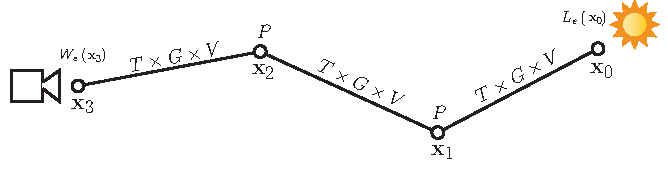
\includegraphics[width=1.0\textwidth]{03_foundations_of_light_transport_simulation/figures/fig_path_sample.pdf}
\caption{Path sample and its contributing factors to energy loss of radiant energy from the light source to the sensor.}
\label{fig:mc_path_sample_contributions}
\end{figure}

Energy is reduced for each segment $\vec{x}_i \vec{x}_{i+1}$ by the geometry term $G$ which results from radiance being defined in terms of the change in projected area, the transmittance term $T$ which accounts for absorption and outscattering and the visibility term $V$ which accounts for geometry obstructing the path alltogether. At each interior path vertex $\vec{x}_i$ scattering is accounted for by multiplying with $p(\vec{x}_i)$. Finally an importance weight $W_e$ accounts for sensor sensitivity.
\begin{align}
f\left(\bar{\mathrm{x}}\right) =
L_e\left(\vec{x}_0\right)
W_e\left(\vec{x}_N\right)
\prod_{i=0}^{i=N-1}
G\left(\vec{x}_i, \vec{x}_{i+1}\right)
T\left(\vec{x}_i, \vec{x}_{i+1}\right)
V\left(\vec{x}_i, \vec{x}_{i+1}\right)
\prod_{i=1}^{i=N-1}
p\left(\vec{x}_i\right)
\label{eq:foundations_mc_pathintegral}
\end{align}
The transmittance is defined as
\begin{align}
T\left(\vec{x}_i, \vec{x}_{i+1}\right) =
\operatorname{exp}^
{
    -\int_{\vec{x}_i}^{\vec{x}_{i+1}}\sigma_t\left(\vec{x}\right)\ud\vec{x}
}
\end{align}
and the geometry term is defined as
\begin{align}
G\left(\vec{x}_i, \vec{x}_{i+1}\right) =
\frac{D\left(\vec{x}_{i}, \vec{x}_{i+1}\right)D\left(\vec{x}_{i+1}, \vec{x}_{i}\right)}{\norm{\vec{x}_{i+1}-\vec{x}_{i}}^2}
\end{align}
with
\begin{align}
D\left(\vec{a}, \vec{b}\right) =
\begin{cases}
\abs{\vec{n}_a\cdot\omega_{ab}}, & \text{for $\vec{a}$ being a surface vertex}
\\
1, & \text{for $\vec{a}$ being a volume vertex}
\end{cases}
\end{align}
Here $\vec{n}_a$ is the normal at the surface vertex $\vec{a}$ and $\omega_{ab}$ is the normalized direction vector pointing from vertex $\vec{a}$ to vertex $\vec{b}$.

Lastly the scattering term $p(\vec{x}_i)$ is defined in terms of the phase function $p$ and the function $p_s$ which is accounting for surface scattering.
\begin{align}
p\left(\vec{x}_i\right) =
\begin{cases}
p_s\left(\omega_{x_ix_{i-1}}\cdot\omega_{x_ix_{i+1}}, \vec{n}_i\right), & \text{for $\vec{x}_i$ being a surface vertex}
\\
p\left(\omega_{x_ix_{i-1}}\cdot\omega_{x_ix_{i+1}}\right), & \text{for $\vec{x}_i$ being a volume vertex}
\end{cases}
\end{align}
This thesis exclusively deals with participating media and therefore surface scattering is of no concern.

The set $\mu\left(\bar{\mathrm{x}}\right)$ is the set of all possible photon trajectories which arrive at $\vec{x}$ from direction $\omega$ and start at any light source in the scene. Each sample is assigned a probability density $p\left(\bar{\mathrm{x}}\right)$ according to a sampling method. The aim of light transport simulation is to find a solution for $L(\vec{x}, \omega)$. With the path integral formulation this can be expressed as a Monte-Carlo integral over path space:
\begin{align}
L\left(\vec{x},\omega\right) = E[g] = \int_{\mu\left(\bar{\mathrm{x}}\right)} \frac{f\left(\bar{\mathrm{x}}\right)}{p\left(\bar{\mathrm{x}}\right)}p\left(\bar{\mathrm{x}}\right)
\ud\mu\left(\bar{\mathrm{x}}\right)
\end{align}
This can be estimated using a finite number of samples $X_i$:
\begin{align}
\left<E[g]\right>_N = 
\frac{1}{N}\sum_{i=0}^{N}
g\left(X_i\right)
\approx
L\left(\vec{x},\omega\right)
\end{align}
As mentioned above, the estimation error shows up as image noise (if random samples are independent). It can be shown formally that in order to cut the amount of noise in half, four times the number of samples is needed (see Veach~\cite{VeachThesis97}). This means that for noise-free results a huge number of samples are needed---a significant drawback of Monte-Carlo methods.

\subsubsection*{Variance Reduction}

Reducing the variance of Monte-Carlo estimators and therefore improving the convergence behaviour is the goal of most of the research on non-deterministic rendering methods. The primary strategy for variance reduction is to reduce the deflection or range of values under the integral sign. This is because the variance is driven by the amount the integrated function deviates from its mean over the integrated range.

There are two ways to reduce the amount of variation of the integrand around its mean value. The first is to adjust the sampling strategy such that the probability density function $p\left(x\right)$ correlates with $f\left(x\right)$ as closely as possible. Ideally the probability density function is identical to $f$ up to a normalization factor $c$. This approach is called importance sampling:
\begin{align}
L = E[g] =
\int_{\mu\left(\bar{\mathrm{x}}\right)} \frac{f\left(\bar{\mathrm{x}}\right)}{p\left(\bar{\mathrm{x}}\right)}p\left(\bar{\mathrm{x}}\right)
\ud\mu\left(\bar{\mathrm{x}}\right)
\stackrel{p\left(x\right)=c f\left(x\right)}{=}
\frac{1}{c}\int_{\mu\left(\bar{\mathrm{x}}\right)} p\left(\bar{\mathrm{x}}\right)
\ud\mu\left(\bar{\mathrm{x}}\right) = \frac{1}{c}
\end{align}
Clearly such a sampling strategy would have to know the solution $L$ in the first place and therefore is only of theoretical interest. However, if the sampling strategies can account for some factors within $f$, a signficiant improvement in variance can be made. Finding good sampling strategies is a vast research branch in its own right within Monte-Carlo based rendering methods. The simplest form is incremental path construction which starts with an inital vertex either on the light source (light path sampling) or the sensor (eye path sampling) and incrementally samples additional points from which additional path segments are constructed. The random decisions are taken according to the terms in $f$ (see equation~\ref{eq:foundations_mc_pathintegral}). The probability density function is constructed by chaining the conditional probabilities for each decision made along the path. This causes the probability density function to respect individual terms and better correlate with the final contribution. 

However, sampling according to individual terms does not respect the product of those terms and therefore is not optimal. This is a continuing subject of research. The basic incremental path sampling was extended by Lafortune et al.~\cite{Lafortune93} and Veach et al.~\cite{Veach94} to bi-directional path-tracing. Here two paths are constructed incrementally. One starts at the light source and the second at the camera sensor. From these two paths multiple individual full paths were constructed and their contribution combined in order to reduce variance. This concept was later generalized by Veach et al.~\cite{Veach95MIS} into multiple importance sampling. It allowed to combine different Monte-Carlo estimators optimized for different light transport aspect. This spurred an explosion of research into sampling techniques and strategies.

Instead of incrementally sampling local terms such as phase function and geometry term to construct the next path vertex, globally informed sampling techniques appear to be a promising avenue. These techniques work by using an approximation to the radiance field function for importance sampling and therefore produce better variance reduction than just using local information at each path vertex. Methods differentiate in their caching datastructure (Gaussian-Mixture Models are used by Vorba et al.~\cite{Vorba14} and an adaptive spatial-directional tree datastructure by M\"{u}ller et al.~\cite{Mueller17}) and the way these caches are bootstrapped (update from Monte-Carlo samples during rendering is done by Vorba et al.~\cite{Vorba14} and reinforcement learning is used by M\"{u}ller et al.~\cite{Mueller17}). These methods are a strong motivation for the use of fast approximative solutions from deterministic methods which are the topic of this thesis. Instead of using expensive unbiased Monte-Carlo samples which are then discretized into a cache datastructure, an approximate solution from a deterministic method could be used to quickly learn the skeleton of light transport in the scene and bootstrap the cache.

The second popular variance reduction technique for Monte-Carlo path tracing is based on control variates. Here the idea is to reduce the deflection of the integrand by using a closed form solution $C$ of an approximation $c\left(x\right)$ to the function $f\left(x\right)$:
\begin{align}
L &= E[g] =
\int_{\mu\left(\bar{\mathrm{x}}\right)}
\frac{f\left(\bar{\mathrm{x}}\right)-c\left(\bar{\mathrm{x}}\right)}{p\left(\bar{\mathrm{x}}\right)}p\left(\bar{\mathrm{x}}\right)
\ud\mu\left(\bar{\mathrm{x}}\right)
+C\left(\vec{x}, \omega\right)
\\
C\left(\vec{x}, \omega\right) &= 
\int_{\mu\left(\bar{\mathrm{x}}\right)}
c\left(\bar{\mathrm{x}}\right)
\ud\mu\left(\bar{\mathrm{x}}\right)
\end{align}
In the ideal case of $c=f$ the integral becomes zero and the equation reduces to $L=C$. Again this would require a closed-form solution of the original problem which does not exist. However, if $c$ correlates well with $f$, variance can be reduced. If no closed form solution for $C$ exists, it can also be integrated numerically using Monte-Carlo integration. Applying the control variates to the integration of $C$ in such a nested fashion yields multilevel Monte-Carlo methods which have not been applied in rendering yet. 

Control variates have been used for surface rendering by Mehta et al.~\cite{Mehta12} and Clarberg et al.~\cite{Clarberg08}. For rendering of participating media control variates have been applied successfully by Pegoraro et al.~\cite{Pegoraro08} where individual samples are used to create and update an adaptive cache of the discretized five-dimensional radiance field. This is very similar to the path-guiding techniques mentioned earlier with the difference that here the guiding cache is used as a control variate instead of a sampling function in the estimator. This work is likewise a good motivation for the deterministic methods developed as part of this thesis. Instead of building the cache from unbiased Monte-Carlo samples and introducing error by discretization into a cache datastructure, an approximation from deterministic methods could be used to bootstrap the cache.

More advanced variance reduction techniques work by better exploring the sample space $\mu\left(x\right)$. Markov-Chain-Monte-Carlo based methods start with a sample which has been generated using standard sampling and from there explore the sampling space by perturbation of that single sample. This concept has been further extended with Hamiltonian Monte-Carlo, where newton dynamics are used to generate trajectories which efficiently explore the important regions in high dimensional sample space. This requires sample space gradients which is a challenge due to the discontinuous visibility function. Coverage of these techniques is far beyond the scope of this thesis. The reader is referred to the work by Veach~\cite{VeachThesis97} and Cline et al.~\cite{Cline05, Cline05apractical} as a starting point into Markov-Chain-Monte-Carlo and the work by Li et al.~\cite{Li15} as an entry point into the use Hamiltonian Monte-Carlo for rendering.

The growth in compute power and the never ending need for more realistic imagery played into the fact that Monte-Carlo methods much better deal with higher dimensions and can produce unbiased result. As in other fields, Monte-Carlo methods are now the gold standard for light transport simulation in computer graphics and improving their convergence is the primary research challenge.

The variance reduction techniques have been presented in this section because they show that having an approximation of the radiance function could be used with importance sampling and control variates to reduce the variance of Monte-Carlo estimators. This is a strong motivation for the use of fast approximative solutions from deterministic methods which will be discussed in the next section and are the topic of this thesis.


% hybrid methods
% Premože et al. proposed a sound mathematically-based version of this approach in the form of the most probable paths most probable (MPP) [PAS03, PAT+04] (bothours thesis p.87) \cite{Premoze04}
%\todo[inline]{Anton Bouthours stuff}
% granular media stuff to show the coupling between diffusion and monte carlo

% hybrid methods: path guiding
% russian roulette and splitting \cite{Vorba16}
% importance sampling \cite{Mueller17}
% propose deterministic methods as initial guide (discuss discretization etc.)



%\todo[inline]{explain the concept of variance}
%\todo[inline]{explain the concept of bias}
%\subsection{Variance Reduction Techniques}
%\label{sec:variance_reduction_techniques}
%\todo[inline]{Explain, that a great variety of Monte Carlo methods exist because there are many ways information and assumptions can be combined with the basic variance reduction techniques available for monte carlo integration}
%\todo[inline]{Local variance reduction technique}
%\todo[inline]{semi-global reduction technique}
%\todo[inline]{global reduction technique}
%\subsubsection{Importance Sampling}
%\todo[inline]{explain importance sampling basics}
%\todo[inline]{multiple importance sampling}
%\todo[inline]{explain JIS as a semi-global technique}
%\todo[inline]{explain SNEE as a semi-global technique}
%\subsubsection{Control Variates}
%\todo[inline]{explain control variates}
%\todo[inline]{multi-level monte carlo}
%\todo[inline]{residual ratio tracking (precomputing the maximum volume height for volume bricks as semi-global))}
%\subsubsection{Russian Roulette and Splitting}
%\todo[inline]{Point out, }
%\todo[inline]{Point out, that the different variance reduction techniques all }

% ============================================================
\section{Deterministic Methods}
\label{sec:foundations_deterministic}

Deterministic methods are based on the discretization of functions which depend on the continuous variables $\vec{x}$ and $\omega$ into a discrete set of scalar values which are flattened into a column vector $\vec{u}$. The discretization operator in angular domain is denoted $\mathcal{P}_\omega$ and the spatial discretization operator is expressed as $\mathcal{P}_{\vec{x}}$
\begin{align*}
L\left(\vec{x}, \omega\right)
\xrightarrow[\mathcal{P}_\omega]{\makebox[1cm]{}}
\xrightarrow[\mathcal{P}_{\vec{x}}]{\makebox[1cm]{}}
\vec{u}
\end{align*}
The discretization operators are also applied to the individual operators $\mathcal{T}$, $\mathcal{C}$ and $\mathcal{S}$ which constitute the radiative transfer equation, producing operator matrices $T$, $C$ and $S$ respectively:
\begin{align*}
\mathcal{T}
\xrightarrow[\mathcal{P}_\omega]{\makebox[1cm]{}}
\xrightarrow[\mathcal{P}_{\vec{x}}]{\makebox[1cm]{}}
T
\\
\mathcal{C}
\xrightarrow[\mathcal{P}_\omega]{\makebox[1cm]{}}
\xrightarrow[\mathcal{P}_{\vec{x}}]{\makebox[1cm]{}}
C
\\
\mathcal{S}
\xrightarrow[\mathcal{P}_\omega]{\makebox[1cm]{}}
\xrightarrow[\mathcal{P}_{\vec{x}}]{\makebox[1cm]{}}
S
\end{align*}
If linear, these discretizations allow to express the application of the radiative transfer operators to the radiance field (see equation~\ref{eq:rte_operator_notation}) to be expressed in terms of matrix vector products:
\begin{align*}
T\vec{u}&=-C\vec{u}+S\vec{u}+Q
\\
T\vec{u}+C\vec{u}-S\vec{u}&=Q
\\
(T+C-S)\vec{u}&=Q
\\
A\vec{u}&=Q
\end{align*}
Deterministic methods turn the problem of solving the radiative transfer equation into the problem of solving a system of linear equations with the solution vector being a discretized version of the radiance field $L$.

The particular choice of $\mathcal{P}_{\vec{x}}$ and $\mathcal{P}_\omega$ determines the concrete method used. For the spatial discretization $\mathcal{P}_{\vec{x}}$ a common choice in nuclear sciences are finite elements and hexagonal meshes in particular, because it allows to best approximate solid geometry (e.g. from reactors) for boundary conditions. However, finite element discretization is unwieldy and difficult to setup. Throughout this theses we use a finite difference discretization which is very common in graphics and also easy to work with in a practical context.
%https://en.wikipedia.org/wiki/Types_of_mesh
%\TD{talk about discretization and meshing}
%\todo[inline]{Spatial Discretization}
%\todo[inline]{Finite differences}
%\todo[inline]{Finite elements}

\subsubsection*{Spherical Harmonics Methods}
%PN
Using the spherical harmonics expansion for the discretization of the radiative transfer equation is a very popular branch of deterministic methods in other fields. Functions which depend on the angular variable are turned into a discrete set of spherical harmonics coefficients. Likewise the radiative transfer equation is turned into a coupled set of partial differential equations through spherical harmonics projection yielding the general $P_N$-equations. The underlying theory has its origins in astrophysics (see Brunner~\cite{Brunner02}) and is also popular in nuclear sciences (see Seibold et al.~\cite{Seibold14}) and medical science (see Frank et al.\cite{Frank08}). In computer graphics $P_N$-theory was discussed briefly in a paper by Kajia~\cite{Kajiya84} without any details on how to solve the equations. In fact, as Max~\cite{Max95} pointed out, it is not clear if Kajiya succeeded at all at implementing a method for solving the $P_N$-equations, as all of the results in his paper were produced with a simpler approach\footnote{\cite{Max95} p.4: \emph{``[...] Kajiya attempted to solve these equations for the case of isotropic scattering, but it is unclear whether he succeeded, since all the pictures in \cite{Kajiya84} were produced by the simpler 'slab' method.[...]"}}. In this thesis we derive the real-valued $P_N$-equations and present a new method for solving them on a finite difference grid. 

The $P_N$-theory has spurred the developement of a rich variety of methods in other domains of which only the diffusion approximation has been introduced into the field of computer graphics (see Stam~\cite{Stam95}). It is derived as a degenerated case of the $P_N$-equations and gained a lot of popularity in graphics. Wang et al.~\cite{Wang08} applied diffusion to the problem of rendering subsurface scattering with heterogeneous particpating media using finite elements. This approach was further extended to anisotropic media by Jakob et al.~\cite{Jakob10} who also used a more complex finite-element discretization in spatial domain. Arbree et al.~\cite{Arbree11} later in a similar approach addressed various problems in Wang's work and simplified discretization by using a tetrahedral mesh basis. Li et al.~\cite{Li13} used the same tetrahedral representation but a more efficient method for constructing the coefficient matrix which allowed realtime application under changing topology.

Another method which is being derived from the spherical harmonics expansion and which can be seen as an extension to the classical diffusion approximation is flux-limited diffusion. The theory has been invented in the astrophysics domain and is primarily attributed to Levermore et al.~\cite{Levermore81}. In computer graphics a method which has some resemblance to flux-limited diffusion in that light transport is modelled as a combination of diffusion and advection has been presented by Zhang et al.~\cite{Zhang13}. In contrast to flux-limited diffusion, their approach is based on ad-hoc assumptions and was not derived formally from the radiative transfer equation. It further works with time-dependent problems and uses a time stepping scheme involving alternating diffusion and advection steps using arbitrary time step and duration parameters. In this thesis, we introduce flux-limited diffusion to the problem of rendering in computer graphics and present a new and efficient method for solving the flux-limited diffusion equation for steady-state radiative transfer.

The purpose of this thesis is to introduce the class of spherical harmonics methods to computer graphics and investigate their merit for applications in rendering. The theory for each method is derived from the spherical harmonics expansion and a solver for practical applications is devised. This includes the $P_N$-method (chapter~\ref{sec:pnmethod}) and flux-limited diffusion (chapter~\ref{sec:fld}). Although classical diffusion already has been introduced to graphics, it is revisited in chapter~\ref{sec:diffusion_approximation} because its theory is important for the introduction of flux-limited diffusion and the multigrid diffusion solver presented has not been discussed in detail in the literature before.

\subsubsection*{Discrete Ordinate Method ($S_N$-Method)}
% SN
Instead of using the continuous spherical harmonics basis functions, an alternative approach for the discretization $\mathcal{P}_\omega$ is to replace the continuous variable $\omega$ by a discrete set of direction vectors $\omega_i$ (e.g. using Gaussian quadrature points) which causes the inscattering integral (equation~\ref{eq:rte_inscattering}) to turn into a sum and in the end produces a system of linear equations. Usually in other fields the variable $s$ is used to identify the direction vector and the discrete directions are denoted $s_i$. This is why the method is also referred to as $S_N$-method (with $N$ being the number of directions). Development of the method is mostly attributed to Wick~\cite{Wick43} and Chandrasekhar~\cite{Chandrasekhar60} who derived the $S_N$-method in one dimension. Later Carlson et al.~\cite{Carlson61} extended the method to two and three dimensions. For the one-dimensional case it has been shown, that $S_{N+1}$-theory is equivalent to $P_N$-theory if Gaussian quadrature points are used (see~\cite{Cullen01}). In this case, the discrete $S_N$-directions correspond to the zero crossings of the Legendre polynomials used in $P_N$. In two or three dimensions however, this correspondence is broken and causes non-physical results, such as the ray effects for which the $S_N$-method is known for.

Like the $P_N$-method, the $S_N$ method also has not been fully explored in the context of rendering in computer graphics yet. Most related is work by Max~\cite{Max95} who introduced a method for computing light propagation in participating media based on directional bins in a regular grid in some way resembling discrete ordinates.


\subsubsection*{Lattice-Boltzmann Method}

The Lattice-Boltzmann method was introduced by Geist et al.~\cite{Geist04} as an alternative to finite-element and finite difference methods for solving partial differential equations. The idea is to simulate transport by tracing evolution of particle distributions through updates on a discrete grid. The iterative step for finding the solution is based on simple voxel update rules which are simple to implement. However, the method hardly got traction as there is no directional resolution but only photon densities per voxel. In addition the formal derivation of the method from the radiative transfer equation is tedious.

\subsubsection*{Heuristical Methods}

The lack of excessive compute power and the need for realtime performance in graphics gave rise to methods which have not been derived formally from radiative transfer and which take additional assumptions to allow further simplification.

Miller et al.~\cite{Miller12} present a method for computing multiple scattering in clouds which seperates the cloud into directly illuminated boundary parts facing the lightsource and a remaining indirectly illuminated part. For the whole dataset the distance function to the directly illuminated part is computed. This requires solving the Eikonal equation using the fast marching method (see~\cite{Tsitsiklis95}). Then the amount of light reaching each point within the medium is computed as a function of distance. While being a crude simplification, the method allows for art-directabiltiy through customizeable radiance-distance profiles.

Light Propagation Volumes by Kaplanyan et al.~\cite{Kaplanyan10} were orginally developed for surface geometry only and have later been extended to participating media by Billeter et al.~\cite{Billeter12}. The scene is aligned with a regular grid where each voxels contains a truncated spherical harmonics expansions of the radiance field (similar to $P_N$). Light emission is computed from single scattered light using reflective shadow maps by Dachsbacher et al.~\cite{Dachsbacher05}. Indirect light is computed by an iterative method. For each iteration, the light at every voxel is distributed to all voxels in a local neighbourhood. The exchange of light is computed for each neighbouring voxel taking the projected surface area of voxel faces into acconut. The process of updating all neighbouring voxels within a certain radius using the light at the center voxel has some resemblance of wavefronts being emitted from the voxel. Although the technique is not derived directly from radiative transfer, it became very popular with realtime rendering for its convincing results.

%\todo[inline]{mention isotropic medium, anisotropic medium}

\begin{figure}[t]
\centering
%\missingfigure{overview of all angular discretization methods.}
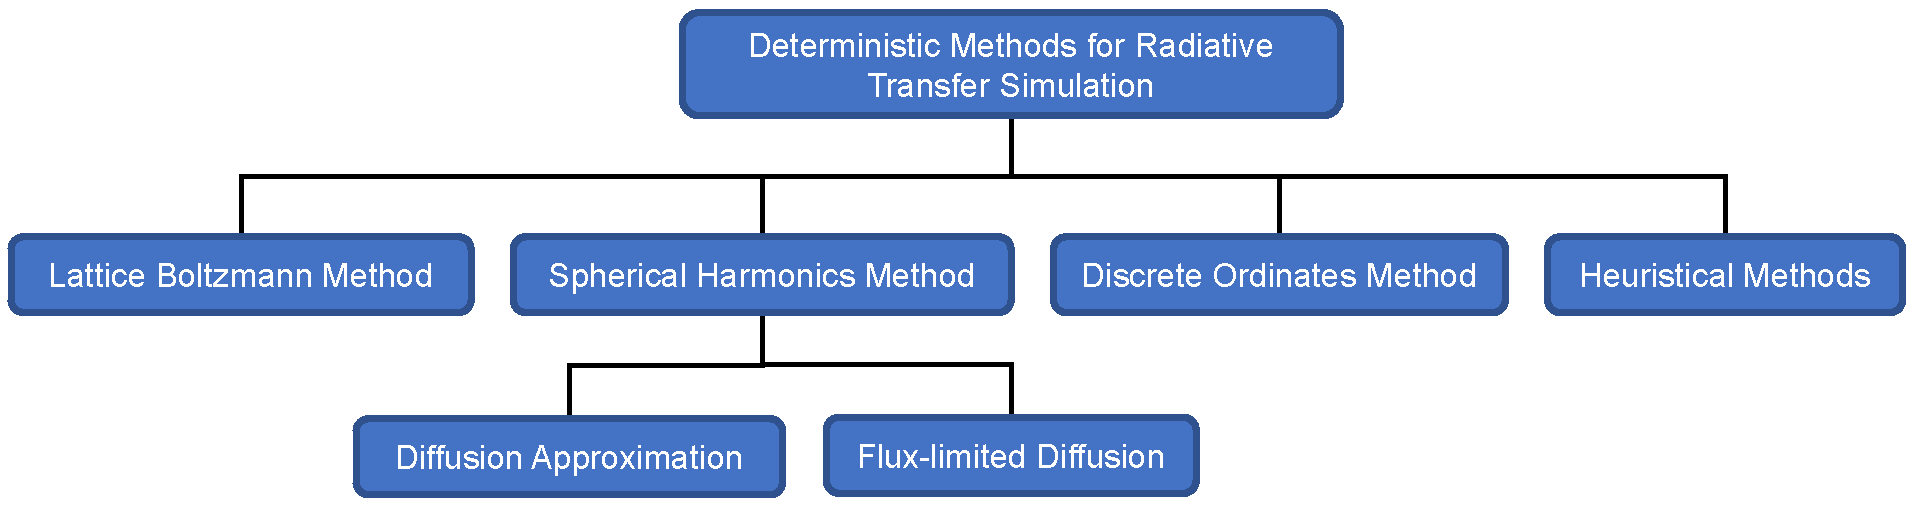
\includegraphics[width=1.0\textwidth]{03_foundations_of_light_transport_simulation/figures/fig_overview_methods.pdf}
\caption{Overview of deterministic methods for light transport simulation.}
\label{fig:rte_change_L_all}
\end{figure}

The benefits of deterministic methods generally are that they provide a noise-free solution for the complete radiance field $L$ throughout the whole domain. Its main drawbacks are their significant memory requirements from storing the representation for the five-dimensional radiance field function and the discretization error from spatial and angular discretization. Further deterministic methods tend to not be as general as Monte-Carlo methods and are limited to a subset of problems (e.g. isotropic phase functions). Additionally some deterministic methods take a lot of time to converge to a solution in certain scenarios.

These drawbacks and the focus on accurate and unbiased Monte-Carlo methods has shifted attention away from deterministic methods lately. However, trends such as the path-guiding techniques discussed in section~\ref{sec:foundations_mc} motivate further research on deterministic methods as they may be useful for bootstrapping guiding caches and therefore could lead to hybrid methods combining the best of both worlds. Consequently, this thesis investigates spherical harmonics methods, the branch of deterministic methods which has seen most popularity in other domains, and tries to asses their merit for applications in rendering.

